\documentclass[main]{subfiles}


\title[AutoML: NAS]{Neural Architecture Search}
\subtitle{One-Shot Techniques in NAS}
\author[Jovita Lukasik]{Jovita Lukasik}
\date{}

\titlebackground*{images/AutoML_NAS}

%\institute{}
%\date{}

\begin{document}
	
	\maketitle
    
%----------------------------------------------------------------------
\begin{frame}{Motivation}
\begin{itemize}
    \item Black-box search strategies train each architecture \alert{independently from scratch} — very expensive
    \item Key insight: architectures in the same search space share \alert{common operations and layers}
    \item Can we exploit this \textbf{structural overlap} to avoid redundant training?
\end{itemize}
\pause
\vspace{0.5em}
\begin{colorblock}[black]{sintefgrey}{Key Question}
Is it possible to train \textbf{all architectures at once} by sharing weights across them — and select the best one without any additional training?
\end{colorblock}		
\end{frame}

\begin{frame}{One-Shot Techniques in Neural Architecture Search}
\begin{center}
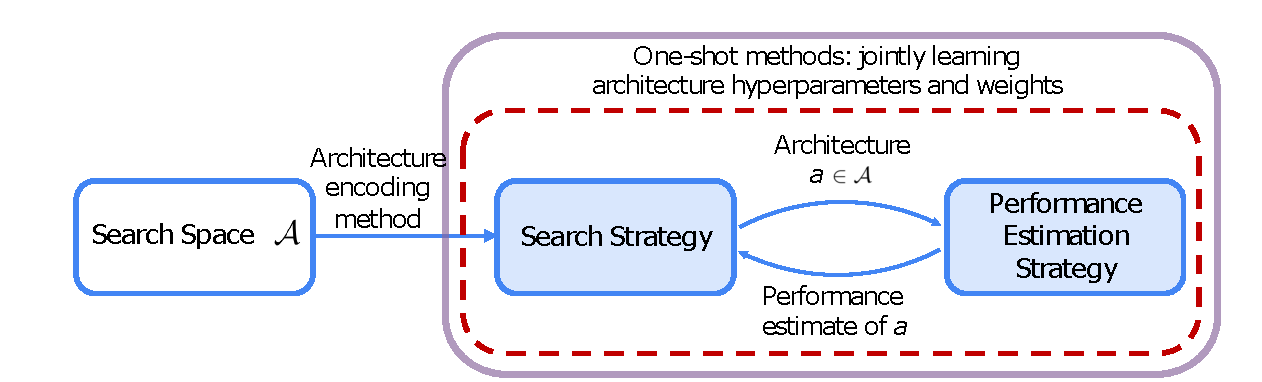
\includegraphics[height=3cm]{images/05/white_2023_nas_overview_4.pdf}
\captionof{figure}{Overview of neural architecture search ~\liturl{White et al. 2023}{https://arxiv.org/pdf/2301.08727.pdf}}
\end{center}
\end{frame}

\begin{frame}{One-Shot Models}
\begin{itemize}
    \item A \alert{one-shot model} (supernet) is a large model that has all architectures in a search space as submodels
    \item This allows \alert{weight sharing} across architectures
    \item One \alert{only needs to train the single one-shot model}, and implicitly trains an exponential number of individual architectures
    \item After training, individual architectures \textbf{inherit} weights from the supernet for evaluation
\end{itemize} 
\end{frame}

% \begin{frame}{Weight-Sharing and One-Shot Techniques}
% The one-shot model can be seen as a directed acyclic multigraph
%     \begin{itemize}
%         \item Nodes: latent representations
%         \item Edges: operations 
%         \item Architecture optimization problem: Find optimal path from input to output
%     \end{itemize}
% \begin{center}
%     
\includegraphics[height=2cm]{images/05/supernet_illustration.pdf}
%     \captionof{figure}{Supernet illustration  ~\liturl{White et al. 2023}{https://arxiv.org/pdf/2301.08727.pdf}}
% \end{center}
    
% \end{frame}

\begin{frame}{One-Shot Models for Cell Search Spaces}
\begin{columns}
    \begin{column}{0.6\textwidth}
    \begin{itemize}
    \item \alert{Directed acyclic multigraph} to capture all (exponentially many) cell architectures	
    \begin{itemize}
	\item The \alert{nodes represent tensors}
	\item The \alert{edges represent computations} 
    \item Results of operations on multiple edges between two nodes are combined (addition / concatenation) 
    \end{itemize}
	\item Individual architectures are subgraphs of this multigraph
    \begin{itemize}
		\item \alert{Weights for the operation on an edge are shared} across all architectures that have that edge
    \end{itemize}
    \item Architecture optimization problem: find the optimal path from input to output
\end{itemize}
        \end{column}
    \begin{column}{0.4\textwidth}
\begin{center}
    
\includegraphics[height=2cm]{images/05/supernet_illustration.pdf}
    \captionof{figure}{Supernet illustration  ~\liturl{White et al. 2023}{https://arxiv.org/pdf/2301.08727.pdf}}
\end{center}
        \end{column}
\end{columns}
\end{frame}

\begin{frame}{One-Shot Model Training -- Standard SGD \liturl{Saxena \& Verbeek. 2017}{https://arxiv.org/pdf/1606.02492.pdf}}
    %Standard SGD ~
    \begin{itemize}
        \item One-shot model is an acyclic graph; backpropagation applies directly
        \begin{itemize}
			\item Simplest method: standard training with SGD
			\item This implicitly trains \alert{an exponential number of architectures}
        \end{itemize}
		\item Potential issue: \textbf{co-adaptation of weights}
        \begin{itemize}
			\item Weights are implicitly optimized to work well \emph{on average} across all architectures
			\item They are \alert{not} optimised specifically for the top-performing architecture
            
        \end{itemize}
    \end{itemize}	
    				
\end{frame}

\begin{frame}{One-Shot Model Training -- DropPath \liturl{Bender et al. 2018}{http://proceedings.mlr.press/v80/bender18a/bender18a.pdf}}
\begin{columns}
    \begin{column}{0.48\textwidth}
    \begin{itemize}
        \item To avoid co-adaptation, apply \alert{DropPath}: analogous to Dropout~\liturl{Srivastava et al. 2014}{http://jmlr.org/papers/v15/srivastava14a.html}
        \begin{itemize}
            \item At each mini-batch iteration: for each operation edge, zero it out with probability $p$
            \item Forces each path to learn independently
        \end{itemize}
        \item \alert{ScheduledDropPath}: start with $p\!=\!0$; increase $p$ linearly to $p_{\max}$ over training
        \begin{itemize}
            \item Gentle regularisation early; stronger later
        \end{itemize}
    \end{itemize}
    \end{column}
    \begin{column}{0.48\textwidth}
    \begin{center}
        

\tikzset{every picture/.style={line width=0.75pt}} %set default line width to 0.75pt        

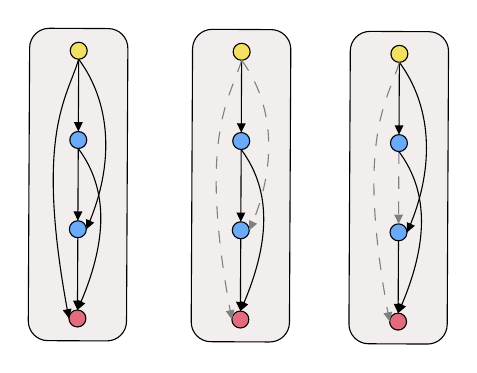
\begin{tikzpicture}[x=0.75pt,y=0.75pt,yscale=-1,xscale=1, scale=0.5]
%uncomment if require: \path (0,354); %set diagram left start at 0, and has height of 354

%Rounded Rect [id:dp4208895880037362] 
\draw  [fill={rgb, 255:red, 242; green, 238; blue, 238 }  ,fill opacity=1 ] (143.14,6.33) .. controls (153.6,6.38) and (162.03,14.9) .. (161.98,25.35) -- (160.7,288.48) .. controls (160.64,298.94) and (152.13,307.38) .. (141.67,307.32) -- (84.87,307.05) .. controls (74.41,307) and (65.98,298.48) .. (66.03,288.02) -- (67.32,24.89) .. controls (67.37,14.43) and (75.88,6) .. (86.34,6.05) -- cycle ;
%Shape: Circle [id:dp4908605297118057] 
\draw  [color={rgb, 255:red, 0; green, 0; blue, 0 }  ,draw opacity=1 ][fill={rgb, 255:red, 243; green, 223; blue, 97 }  ,fill opacity=1 ] (114.68,19.52) .. controls (119.19,19.54) and (122.83,23.21) .. (122.81,27.73) .. controls (122.79,32.24) and (119.11,35.88) .. (114.6,35.86) .. controls (110.08,35.84) and (106.44,32.16) .. (106.46,27.65) .. controls (106.48,23.13) and (110.16,19.49) .. (114.68,19.52) -- cycle ;
%Shape: Circle [id:dp32910894757430365] 
\draw  [fill={rgb, 255:red, 105; green, 170; blue, 249 }  ,fill opacity=1 ] (114.26,105.51) .. controls (118.77,105.54) and (122.41,109.21) .. (122.39,113.73) .. controls (122.37,118.24) and (118.69,121.88) .. (114.18,121.86) .. controls (109.66,121.84) and (106.02,118.16) .. (106.04,113.65) .. controls (106.06,109.13) and (109.74,105.49) .. (114.26,105.51) -- cycle ;
%Shape: Circle [id:dp39694232134723384] 
\draw  [fill={rgb, 255:red, 105; green, 170; blue, 249 }  ,fill opacity=1 ] (113.84,191.51) .. controls (118.35,191.54) and (121.99,195.21) .. (121.97,199.73) .. controls (121.95,204.24) and (118.27,207.88) .. (113.76,207.86) .. controls (109.24,207.84) and (105.6,204.16) .. (105.62,199.65) .. controls (105.64,195.13) and (109.32,191.49) .. (113.84,191.51) -- cycle ;
%Shape: Circle [id:dp05994064859317039] 
\draw  [fill={rgb, 255:red, 228; green, 107; blue, 124 }  ,fill opacity=1 ] (113.41,277.51) .. controls (117.93,277.53) and (121.57,281.21) .. (121.55,285.73) .. controls (121.53,290.24) and (117.85,293.88) .. (113.34,293.86) .. controls (108.82,293.84) and (105.18,290.16) .. (105.2,285.65) .. controls (105.22,281.13) and (108.9,277.49) .. (113.41,277.51) -- cycle ;
%Straight Lines [id:da13324796783877657] 
\draw    (114.6,35.86) -- (114.27,102.51) ;
\draw [shift={(114.26,105.51)}, rotate = 270.28] [fill={rgb, 255:red, 0; green, 0; blue, 0 }  ][line width=0.08]  [draw opacity=0] (8.93,-4.29) -- (0,0) -- (8.93,4.29) -- cycle    ;
%Straight Lines [id:da45435201736948916] 
\draw    (114.18,121.86) -- (113.85,188.51) ;
\draw [shift={(113.84,191.51)}, rotate = 270.28] [fill={rgb, 255:red, 0; green, 0; blue, 0 }  ][line width=0.08]  [draw opacity=0] (8.93,-4.29) -- (0,0) -- (8.93,4.29) -- cycle    ;
%Straight Lines [id:da4152608208525701] 
\draw    (113.76,207.86) -- (113.43,274.51) ;
\draw [shift={(113.41,277.51)}, rotate = 270.28] [fill={rgb, 255:red, 0; green, 0; blue, 0 }  ][line width=0.08]  [draw opacity=0] (8.93,-4.29) -- (0,0) -- (8.93,4.29) -- cycle    ;
%Curve Lines [id:da10478213596403207] 
\draw    (114.6,35.86) .. controls (144.1,75.61) and (151,133.69) .. (122.83,197.78) ;
\draw [shift={(121.97,199.73)}, rotate = 294.21] [fill={rgb, 255:red, 0; green, 0; blue, 0 }  ][line width=0.08]  [draw opacity=0] (8.93,-4.29) -- (0,0) -- (8.93,4.29) -- cycle    ;
%Curve Lines [id:da9168131818811978] 
\draw    (114.18,121.86) .. controls (143.68,161.61) and (142.6,211.64) .. (114.28,275.57) ;
\draw [shift={(113.41,277.51)}, rotate = 294.21] [fill={rgb, 255:red, 0; green, 0; blue, 0 }  ][line width=0.08]  [draw opacity=0] (8.93,-4.29) -- (0,0) -- (8.93,4.29) -- cycle    ;
%Curve Lines [id:da1366332199563608] 
\draw    (114.6,35.86) .. controls (103.49,73.44) and (71.58,108.12) .. (104.7,283) ;
\draw [shift={(105.2,285.65)}, rotate = 259.16] [fill={rgb, 255:red, 0; green, 0; blue, 0 }  ][line width=0.08]  [draw opacity=0] (8.93,-4.29) -- (0,0) -- (8.93,4.29) -- cycle    ;

%Rounded Rect [id:dp17154346128785647] 
\draw  [fill={rgb, 255:red, 242; green, 238; blue, 238 }  ,fill opacity=1 ] (300.14,7.33) .. controls (310.6,7.38) and (319.03,15.9) .. (318.98,26.35) -- (317.7,289.48) .. controls (317.64,299.94) and (309.13,308.38) .. (298.67,308.32) -- (241.87,308.05) .. controls (231.41,308) and (222.98,299.48) .. (223.03,289.02) -- (224.32,25.89) .. controls (224.37,15.43) and (232.88,7) .. (243.34,7.05) -- cycle ;
%Shape: Circle [id:dp9509110800564388] 
\draw  [color={rgb, 255:red, 0; green, 0; blue, 0 }  ,draw opacity=1 ][fill={rgb, 255:red, 243; green, 223; blue, 97 }  ,fill opacity=1 ] (271.68,20.52) .. controls (276.19,20.54) and (279.83,24.21) .. (279.81,28.73) .. controls (279.79,33.24) and (276.11,36.88) .. (271.6,36.86) .. controls (267.08,36.84) and (263.44,33.16) .. (263.46,28.65) .. controls (263.48,24.13) and (267.16,20.49) .. (271.68,20.52) -- cycle ;
%Shape: Circle [id:dp8778742410693867] 
\draw  [fill={rgb, 255:red, 105; green, 170; blue, 249 }  ,fill opacity=1 ] (271.26,106.51) .. controls (275.77,106.54) and (279.41,110.21) .. (279.39,114.73) .. controls (279.37,119.24) and (275.69,122.88) .. (271.18,122.86) .. controls (266.66,122.84) and (263.02,119.16) .. (263.04,114.65) .. controls (263.06,110.13) and (266.74,106.49) .. (271.26,106.51) -- cycle ;
%Shape: Circle [id:dp635233862148283] 
\draw  [fill={rgb, 255:red, 105; green, 170; blue, 249 }  ,fill opacity=1 ] (270.84,192.51) .. controls (275.35,192.54) and (278.99,196.21) .. (278.97,200.73) .. controls (278.95,205.24) and (275.27,208.88) .. (270.76,208.86) .. controls (266.24,208.84) and (262.6,205.16) .. (262.62,200.65) .. controls (262.64,196.13) and (266.32,192.49) .. (270.84,192.51) -- cycle ;
%Shape: Circle [id:dp6064891340021821] 
\draw  [fill={rgb, 255:red, 228; green, 107; blue, 124 }  ,fill opacity=1 ] (270.41,278.51) .. controls (274.93,278.53) and (278.57,282.21) .. (278.55,286.73) .. controls (278.53,291.24) and (274.85,294.88) .. (270.34,294.86) .. controls (265.82,294.84) and (262.18,291.16) .. (262.2,286.65) .. controls (262.22,282.13) and (265.9,278.49) .. (270.41,278.51) -- cycle ;
%Straight Lines [id:da9015554562598511] 
\draw    (271.6,36.86) -- (271.27,103.51) ;
\draw [shift={(271.26,106.51)}, rotate = 270.28] [fill={rgb, 255:red, 0; green, 0; blue, 0 }  ][line width=0.08]  [draw opacity=0] (8.93,-4.29) -- (0,0) -- (8.93,4.29) -- cycle    ;
%Straight Lines [id:da38844208885435316] 
\draw    (271.18,122.86) -- (270.85,189.51) ;
\draw [shift={(270.84,192.51)}, rotate = 270.28] [fill={rgb, 255:red, 0; green, 0; blue, 0 }  ][line width=0.08]  [draw opacity=0] (8.93,-4.29) -- (0,0) -- (8.93,4.29) -- cycle    ;
%Straight Lines [id:da9143022220153731] 
\draw    (270.76,208.86) -- (270.43,275.51) ;
\draw [shift={(270.41,278.51)}, rotate = 270.28] [fill={rgb, 255:red, 0; green, 0; blue, 0 }  ][line width=0.08]  [draw opacity=0] (8.93,-4.29) -- (0,0) -- (8.93,4.29) -- cycle    ;
%Curve Lines [id:da06811477582899617] 
\draw [color={rgb, 255:red, 128; green, 128; blue, 128 }  ,draw opacity=1 ] [dash pattern={on 4.5pt off 4.5pt}]  (271.6,36.86) .. controls (301.1,76.61) and (308,134.69) .. (279.83,198.78) ;
\draw [shift={(278.97,200.73)}, rotate = 294.21] [fill={rgb, 255:red, 128; green, 128; blue, 128 }  ,fill opacity=1 ][line width=0.08]  [draw opacity=0] (8.93,-4.29) -- (0,0) -- (8.93,4.29) -- cycle    ;
%Curve Lines [id:da08351144146888023] 
\draw    (271.18,122.86) .. controls (300.68,162.61) and (299.6,212.64) .. (271.28,276.57) ;
\draw [shift={(270.41,278.51)}, rotate = 294.21] [fill={rgb, 255:red, 0; green, 0; blue, 0 }  ][line width=0.08]  [draw opacity=0] (8.93,-4.29) -- (0,0) -- (8.93,4.29) -- cycle    ;
%Curve Lines [id:da6747987338076401] 
\draw [color={rgb, 255:red, 128; green, 128; blue, 128 }  ,draw opacity=1 ] [dash pattern={on 4.5pt off 4.5pt}]  (271.6,36.86) .. controls (260.49,74.44) and (228.58,109.12) .. (261.7,284) ;
\draw [shift={(262.2,286.65)}, rotate = 259.16] [fill={rgb, 255:red, 128; green, 128; blue, 128 }  ,fill opacity=1 ][line width=0.08]  [draw opacity=0] (8.93,-4.29) -- (0,0) -- (8.93,4.29) -- cycle    ;
%Rounded Rect [id:dp33927272410791576] 
\draw  [fill={rgb, 255:red, 242; green, 238; blue, 238 }  ,fill opacity=1 ] (452.14,9.33) .. controls (462.6,9.38) and (471.03,17.9) .. (470.98,28.35) -- (469.7,291.48) .. controls (469.64,301.94) and (461.13,310.38) .. (450.67,310.32) -- (393.87,310.05) .. controls (383.41,310) and (374.98,301.48) .. (375.03,291.02) -- (376.32,27.89) .. controls (376.37,17.43) and (384.88,9) .. (395.34,9.05) -- cycle ;
%Shape: Circle [id:dp7211478574824824] 
\draw  [color={rgb, 255:red, 0; green, 0; blue, 0 }  ,draw opacity=1 ][fill={rgb, 255:red, 243; green, 223; blue, 97 }  ,fill opacity=1 ] (423.68,22.52) .. controls (428.19,22.54) and (431.83,26.21) .. (431.81,30.73) .. controls (431.79,35.24) and (428.11,38.88) .. (423.6,38.86) .. controls (419.08,38.84) and (415.44,35.16) .. (415.46,30.65) .. controls (415.48,26.13) and (419.16,22.49) .. (423.68,22.52) -- cycle ;
%Shape: Circle [id:dp002604107977017822] 
\draw  [fill={rgb, 255:red, 105; green, 170; blue, 249 }  ,fill opacity=1 ] (423.26,108.51) .. controls (427.77,108.54) and (431.41,112.21) .. (431.39,116.73) .. controls (431.37,121.24) and (427.69,124.88) .. (423.18,124.86) .. controls (418.66,124.84) and (415.02,121.16) .. (415.04,116.65) .. controls (415.06,112.13) and (418.74,108.49) .. (423.26,108.51) -- cycle ;
%Shape: Circle [id:dp6004551048950394] 
\draw  [fill={rgb, 255:red, 105; green, 170; blue, 249 }  ,fill opacity=1 ] (422.84,194.51) .. controls (427.35,194.54) and (430.99,198.21) .. (430.97,202.73) .. controls (430.95,207.24) and (427.27,210.88) .. (422.76,210.86) .. controls (418.24,210.84) and (414.6,207.16) .. (414.62,202.65) .. controls (414.64,198.13) and (418.32,194.49) .. (422.84,194.51) -- cycle ;
%Shape: Circle [id:dp31886993733122493] 
\draw  [fill={rgb, 255:red, 228; green, 107; blue, 124 }  ,fill opacity=1 ] (422.41,280.51) .. controls (426.93,280.53) and (430.57,284.21) .. (430.55,288.73) .. controls (430.53,293.24) and (426.85,296.88) .. (422.34,296.86) .. controls (417.82,296.84) and (414.18,293.16) .. (414.2,288.65) .. controls (414.22,284.13) and (417.9,280.49) .. (422.41,280.51) -- cycle ;
%Straight Lines [id:da2160398914020527] 
\draw    (423.6,38.86) -- (423.27,105.51) ;
\draw [shift={(423.26,108.51)}, rotate = 270.28] [fill={rgb, 255:red, 0; green, 0; blue, 0 }  ][line width=0.08]  [draw opacity=0] (8.93,-4.29) -- (0,0) -- (8.93,4.29) -- cycle    ;
%Straight Lines [id:da8038843580445767] 
\draw [color={rgb, 255:red, 128; green, 128; blue, 128 }  ,draw opacity=1 ] [dash pattern={on 4.5pt off 4.5pt}]  (423.18,124.86) -- (422.85,191.51) ;
\draw [shift={(422.84,194.51)}, rotate = 270.28] [fill={rgb, 255:red, 128; green, 128; blue, 128 }  ,fill opacity=1 ][line width=0.08]  [draw opacity=0] (8.93,-4.29) -- (0,0) -- (8.93,4.29) -- cycle    ;
%Straight Lines [id:da5117190411103258] 
\draw    (422.76,210.86) -- (422.43,277.51) ;
\draw [shift={(422.41,280.51)}, rotate = 270.28] [fill={rgb, 255:red, 0; green, 0; blue, 0 }  ][line width=0.08]  [draw opacity=0] (8.93,-4.29) -- (0,0) -- (8.93,4.29) -- cycle    ;
%Curve Lines [id:da9507835254277128] 
\draw    (423.6,38.86) .. controls (453.1,78.61) and (460,136.69) .. (431.83,200.78) ;
\draw [shift={(430.97,202.73)}, rotate = 294.21] [fill={rgb, 255:red, 0; green, 0; blue, 0 }  ][line width=0.08]  [draw opacity=0] (8.93,-4.29) -- (0,0) -- (8.93,4.29) -- cycle    ;
%Curve Lines [id:da9972298839164025] 
\draw    (423.18,124.86) .. controls (452.68,164.61) and (451.6,214.64) .. (423.28,278.57) ;
\draw [shift={(422.41,280.51)}, rotate = 294.21] [fill={rgb, 255:red, 0; green, 0; blue, 0 }  ][line width=0.08]  [draw opacity=0] (8.93,-4.29) -- (0,0) -- (8.93,4.29) -- cycle    ;
%Curve Lines [id:da7684695212865164] 
\draw [color={rgb, 255:red, 128; green, 128; blue, 128 }  ,draw opacity=1 ] [dash pattern={on 4.5pt off 4.5pt}]  (423.6,38.86) .. controls (412.49,76.44) and (380.58,111.12) .. (413.7,286) ;
\draw [shift={(414.2,288.65)}, rotate = 259.16] [fill={rgb, 255:red, 128; green, 128; blue, 128 }  ,fill opacity=1 ][line width=0.08]  [draw opacity=0] (8.93,-4.29) -- (0,0) -- (8.93,4.29) -- cycle    ;
\end{tikzpicture}
        % \includegraphics[width=\textwidth]{images/05/droppath_illustration.png}
        \captionof{figure}{DropPath: edges (operations) are randomly zeroed per mini-batch}
    \end{center}
    \end{column}
\end{columns}
\end{frame}

\begin{frame}{One-Shot Model Training -- Sampling}
  \begin{itemize}
    \item \textbf{Uniform sampling — Random Search with Weight Sharing (RSWS)}~\liturl{Li and Talwalkar 2020}{https://arxiv.org/pdf/1902.07638.pdf}
    \begin{itemize}
        \item Each sub-architecture sampled from uniform distribution
        \item Simple and surprisingly competitive
    \end{itemize}
    \item \textbf{Policy-based sampling — ENAS}~\liturl{Pham et al. 2018}{https://arxiv.org/pdf/1802.03268.pdf}
    \begin{itemize}
        \item Sample from the learned policy of an RNN controller
        \item Controller and supernet trained alternately
    \end{itemize}
    \item \textbf{Single-Path One-Shot (SPOS)}~\liturl{Guo et al. 2020}{https://arxiv.org/pdf/1904.00420.pdf}
    \begin{itemize}
        \item Uniform path sampling, then evolutionary search over the trained supernet
        \item Fully decoupled supernet training from architecture search
    \end{itemize}
	\end{itemize}
\end{frame}


%----------------------------------------------------------------------
% WEIGHT ENTANGLEMENT AND FAIRNESS
%----------------------------------------------------------------------

% \begin{frame}{The Weight Entanglement Problem}
% \begin{itemize}
%     \item In uniform sampling, each operation may be sampled at \alert{very different frequencies} depending on the search space structure
%     \item \textbf{Consequence}: some operations receive far more gradient updates than others
%     \item $\rightsquigarrow$ The weights of rarely-sampled operations are \alert{under-trained} relative to frequently-sampled ones
%     \item This \textbf{biases} the supernet's ranking of architectures and reduces ranking correlation with stand-alone performance
% \end{itemize}
% \vspace{0.4em}
% \begin{block}{Weight Entanglement}
%     Shared weights are simultaneously optimised for \emph{all} sub-architectures that use them — which can conflict when sub-architectures require different optimal weight values.
% \end{block}
% \end{frame}

% \begin{frame}{FairNAS — Fair Sampling}
% FairNAS~\liturl{Chu et al. 2021}{https://arxiv.org/abs/1907.01845}
% \begin{itemize}
%     \item Identifies unfairness as the root cause of poor supernet ranking
%     \item \alert{Fair sampling constraint}: each operation (choice block) is sampled equally often per update step
%     \begin{itemize}
%         \item Superimposes gradients from $K$ sub-architectures simultaneously to ensure equal update frequency
%     \end{itemize}
%     \item Reduces the optimisation gap between operations
%     \item Empirically yields significantly \textbf{higher ranking correlation} (Spearman $\rho$) than plain uniform sampling
% \end{itemize}
% \pause
% \vspace{0.3em}
% $\rightsquigarrow$ Fairness in training is \textbf{as important} as the search strategy applied after supernet training
% \end{frame}


\begin{frame}{How to Utilize the Trained One-Shot Model?}
    \begin{itemize}
			\item After training the one-shot model, \alert{select the best individual architecture} from it
		\item Several strategies:
\begin{itemize}
    \item Sample $M$ architectures uniformly at random; rank by validation error \alert{using the supernet weights}
    \item Return the top architecture to \alert{retrain from scratch} for full training
    \item Evolutionary or BO search over the supernet (\textbf{SPOS approach})
\end{itemize}
	\end{itemize}
\begin{columns}
	    \column{0.01\textwidth}
    	\column{0.4\textwidth}
        	\begin{itemize}
				\footnotesize
				\item \textbf{Pitfall:} the correlation between architectures evaluated with the one-shot weights and retrained from scratch (stand-alone models) should be high
				% \item 
                % If not, \textbf{selecting the best architecture based on the one-shot weights} is sub-optimal.
			\end{itemize}
	    \column{0.5\textwidth}
\begin{center}
\vspace*{-0.3cm}
	        
\includegraphics[width=.65\textwidth]{07_NAS/images/05/bender_correlation_1.png}\\
	        \scriptsize{From \smaller{\liturl{Bender et al. 2018}{http://proceedings.mlr.press/v80/bender18a/bender18a.pdf}}}
\end{center}
    	\end{columns}
\end{frame}

\begin{frame}{Ranking Correlation — A Persistent Challenge}
\begin{itemize}
    \item Ranking correlation between supernet and stand-alone models is \alert{often low in practice}~\liturl{Yu et al. 2020}{https://openreview.net/pdf?id=H1loF2NFwr} $\rightsquigarrow$ Ranking Disorder
    \item Causes:
    \begin{enumerate}
        \item Weight co-adaptation / entanglement
        \item Insufficient supernet training
        \item Mismatch between supernet and sub-architecture batch normalisation statistics
    \end{enumerate}
    \item Mitigations:
    \begin{itemize}
        \item \textbf{GreedyNAS}~\liturl{You et al. 2020}{https://openaccess.thecvf.com/content_CVPR_2020/papers/You_GreedyNAS_Towards_Fast_One-Shot_NAS_With_Greedy_Supernet_CVPR_2020_paper.pdf}: introduce multi-path sampling strategy with rejection to filter the weak paths and greedily train potentially-good paths
        \item \textbf{PGONAS}~\liturl{Dong et al. 2022}{https://arxiv.org/pdf/2206.13329}: use zero-cost proxies (Zen-Score, FLOPs) as auxiliary ranking loss during supernet training
        \item \textbf{ShiftNAS}~\liturl{Zhang et al. 2023}{https://openaccess.thecvf.com/content/ICCV2023/papers/Zhang_ShiftNAS_Improving_One-shot_NAS_via_Probability_Shift_ICCV_2023_paper.pdf}: learnable sampling distribution adapts to subnet complexity during training
        \item \textbf{CaLR}~\liturl{Jeon et al. 2025}{https://openaccess.thecvf.com//content/CVPR2025/papers/Jeon_Subnet-Aware_Dynamic_Supernet_Training_for_Neural_Architecture_Search_CVPR_2025_paper.pdf}: adjusting the learning rate based on the complexity of the subnets        
    \end{itemize}
\end{itemize}
\end{frame}


\begin{frame}{Weight-Sharing and One-Shot Techniques}
\begin{itemize}
    \item Once one-shot model trained inherit weight for subnet from supernet 
    \item Scalability and efficiency:
    \begin{itemize}
        \item Linear increase in number of candidates causes linear increase in computational costs for training but number of subnets increases exponentially 
    \end{itemize}
$\rightsquigarrow$ Supernet allows to train exponential number of architectures in linear compute costs
\end{itemize}
\vspace{0.4em}
\alert{Key assumption}: the ranking of architectures under the supernet is relatively consistent with the ranking from independent training

\vspace{0.4em}
The supernet allows quick evaluation, but a \textbf{search strategy is still needed} (either during or after supernet training)
\end{frame}

% \begin{frame}{One-Shot NAS Beyond CNNs — Vision Transformers}
% \begin{itemize}
%     \item Weight-sharing supernets have been extended to \alert{Vision Transformers (ViTs)}
%     \item \textbf{AutoFormer}~\liturl{Chen et al. 2021}{https://arxiv.org/pdf/2107.00651.pdf}
%     \begin{itemize}
%         \item First one-shot NAS method for ViTs using an \alert{Any-Transformer supernet}
%         \item Searches over embedding dimensions, number of heads, MLP ratios, and depth
%         \item Uses \textbf{weight entanglement}: smaller subnets reuse a prefix of the larger supernet's weight matrix
%         \item Decoupled search: supernet trained once; evolutionary search finds the optimal subnet for a given FLOPs constraint
%     \end{itemize}
%     \item Demonstrates that one-shot + weight sharing generalises \textbf{beyond convolutional architectures}
% \end{itemize}
% \end{frame}

% \begin{frame}{One-Shot NAS at Scale — Recent Findings}
% \begin{itemize}
%     \item \textbf{PreNAS}~\liturl{Wang et al. 2023}{https://proceedings.mlr.press/v202/wang23p.html}: search-free NAS — use zero-cost proxies to pre-select a small set of promising architectures, then train only their shared supernet
%     \begin{itemize}
%         \item Reduces update conflicts and improves efficiency significantly
%     \end{itemize}
%     \item \textbf{MoE Supernet}~\liturl{Su et al. 2024}{https://aclanthology.org/2024.acl-long.97.pdf}: mixture-of-experts routing for indirect weight sharing
%     \begin{itemize}
%         \item Architecture-based routing adapts shared weights per subnet, reducing entanglement
%     \end{itemize}
%     \item \textbf{Key finding}~\liturl{Yu et al. 2020}{https://arxiv.org/abs/2007.04010}: on many benchmarks, a carefully trained supernet with uniform sampling and BN recalibration \alert{matches or exceeds} sophisticated RL / BO search strategies at a fraction of the cost
% \end{itemize}
% \end{frame}
%----------------------------------------------------------------------
\begin{frame}{Summary} 

Most important insights from this video:

\begin{enumerate}
    \item All possible architectures are subgraphs of a single large supergraph (one-shot model / supernet), which shares weights across architectures
    \item \textbf{DropPath} and \textbf{ScheduledDropPath} prevent weight co-adaptation by randomly zeroing operation edges during training
    % \item \textbf{Sampling fairness} (FairNAS) is critical: unequal operation frequencies bias the supernet and degrade ranking correlation
    \item Ranking correlation between the supernet and stand-alone models remains a key challenge; ranking-aware losses (PGONAS), and adaptive sampling (ShiftNAS) are recent remedies
    % \item Weight-sharing supernets now extend to Vision Transformers (AutoFormer) and scale to large NLP models via mixture-of-experts routing

\end{enumerate}


\end{frame}



\end{document}
